\documentclass[a4paper]{scrartcl}
\usepackage{amsmath, amsthm, amssymb}
\numberwithin{equation}{section}
\usepackage[T1]{fontenc}
\usepackage[english]{babel}
\usepackage[utf8]{inputenc}
\usepackage[parfill]{parskip}    % Activate to begin paragraphs with an empty line rather than an indent
\usepackage{graphicx}
\usepackage{caption}
\usepackage{subcaption}
\usepackage{wrapfig}
\usepackage{verbatim}
\usepackage{listings}
\usepackage{fancyhdr}
\usepackage{url}
%\usepackage[]{mcode} % \lstinputlisting[firstline=300,lastline=500]{file.m}

% The report should contain:
% 1. A cover sheet with the name of the project, your names, education programs, and e-mail addresses. You must check mail to these addresses regularly.
%    Also give the date of submission and complete instructions for running your program.
% 2. An introduction (what the project is about, etc.).
% 3. Something about requirements that you fulfill or don’t fulfill.
% 4. An outline of your system (which database manager you use, which programs you have
%    written, how the programs communicate with the database, etc.).
% 5. An E/R diagram which describes the system.
% 6. Relations. Indicate primary keys, possibly secondary keys, and foreign keys. You must
%    show that the relations are normalized according to your chosen normal form (if a relation “obviously” is in BCNF you may say so,
%    provided that you  justify your statement). If a relation is in a lower normal form than BCNF, you must justify this choice.
% 7. SQL statements to create all tables, views, stored procedures, and other database elements.
%    (Don’t include statements to create the initial contents of the database.)
% 8. A user’s manual (not necessary if everything in the program is self-explanatory).


\pagestyle{fancy}
\thispagestyle{empty}
\rhead{Johannes Jansson and Victor Miller}
\lhead{}

\begin{document}

\title{Programming Project: Krusty Kookies}
\author{Johannes Jansson, F11\\tfy11jja@student.lu.se\\\\Victor Miller, F11\\tfy11vmi@student.lu.se}

\date{}
\maketitle
\newpage

\section*{Introduction}
The fictive company Krusty Kookies has recently expanded into Sweden, and needs a computerized system for production and delivery of cookies. 
The system needs to handle everything: storage of ingredients, lists of recipes, tracking of pallets, placed orders and deliveries. 
This project is a part of the LTH course EDA216 -- Database technology, and our task is to implement the parts of this system related to production.
We will also create a screen that simulated production, so that the system can be tested without the presence of an actual factory.


\section*{Requirements}
Even though the requirements were a bit diffuse (as intended) we are fairly confident that we have met all of them. 
\section*{Outline of the System}
The system is constructed in a way much similar to the system in lab 4. 
The database manager MySQL is used to manage the database, located on \url{puccini.cs.lth.se}. 
The creation and population of the database is performed by sourcing the file \textbf{tables.sql}, the creation is described in listing \ref{tables.sql}.

The factory interface is a web page written in PHP. 
The php tool PDO was used to establish a connection to the database. 
The PHP class \textbf{database.inc.php} handles everything related to the SQL database, and the PHP class \textbf{pallet.inc.php} is used to transmit data from the database class to the webpage.
The connection is established just as in the lab.
Updates and queries are made using perpared statements:
\begin{verbatim}
$stmt = $this->conn->prepare($query);
$stmt->execute($param);
\end{verbatim}
to protect the database from SQL injections. 
The newly created methods for this assignment are:
\begin{itemize}
  \item \textbf{producePallet(\$date, \$time, \$name)} simulates the production of a pallet.
  \item \textbf{getPallet(\$barcode)} returns a php pallet object with information from the corresponding pallet tuple in Pallets.
  \item \textbf{blockIntervall(\$product, \$date, \$startTime, \$endTime)} finds all pallets meeting the criteria, blocks them and returns them.
  \item \textbf{generalSearch} handles all searching requested by the user.
\end{itemize}
There are also methods for getting all locations, production dates, barcodes and products, used for generating dropdown menus in the user interface. 
The class \textbf{database.inc.php} is quite well commented, have a look there for more details.

The pallet class only consists of variables, a constructor and getters.



The interface consists of 8 views. The first view that the user ecounters is the login page. This is a simple view that only has as purporse to login to to the database. The view can be seen below 

\begin{figure}[h]
  \centering
  	\begin{subfigure}[b]{0.45\textwidth}
    	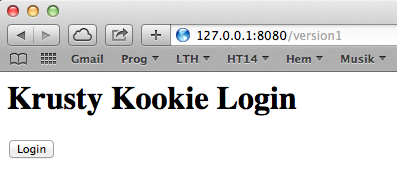
\includegraphics[width=\textwidth]{figures/view_login.png}
    	\label{figure:view_login}
    	\caption{Login view for the interface}
 		\end{subfigure}	
 		\begin{subfigure}[b]{0.45\textwidth}
    	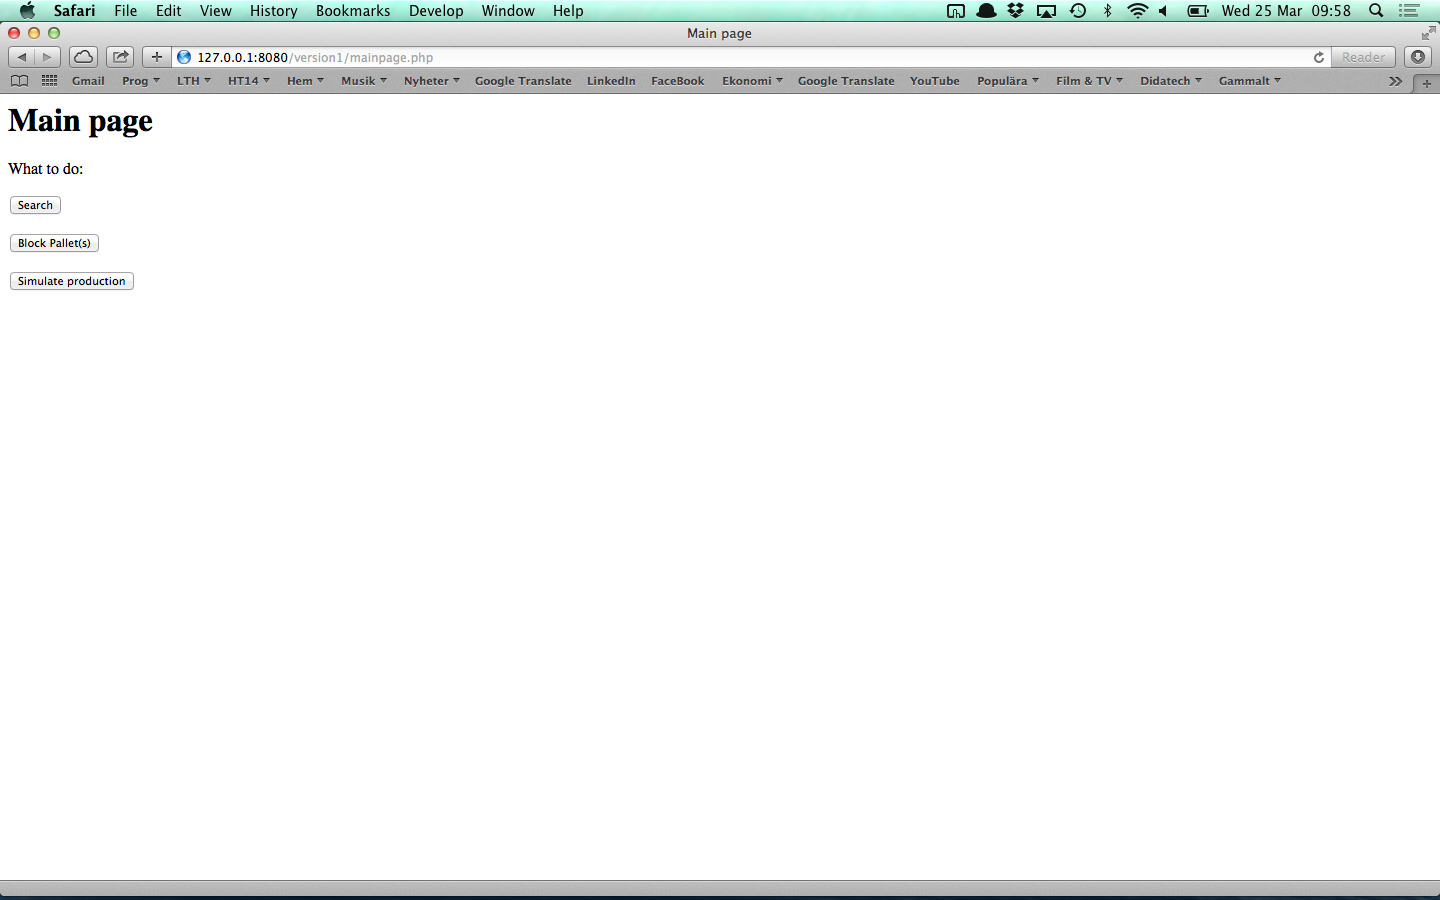
\includegraphics[width=\textwidth]{figures/view_mainpage.png}
    	\label{figure:view_mainpage}
    	\caption{View for the main page}
 		\end{subfigure} 
 		\caption{First views}
\end{figure}

The user can then navigate on to one of the three options given, \emph{Search, Block Pallet(s)} or \emph{Simulate Production}. Each one of them has one input view where the user can provide the program with suitable input and the submit. The user is the provided with a result view to see what happend according to the given input.

\subsection*{Searching}

In the searching view the user can choose to search on different parameters. Each parameter can be left as \emph{All} or set to a specific value. This gives the user the possibility to define thier search as they want. An example of the search view and the result is given below

\begin{figure}[h]
  \centering
  	\begin{subfigure}[b]{0.45\textwidth}
    	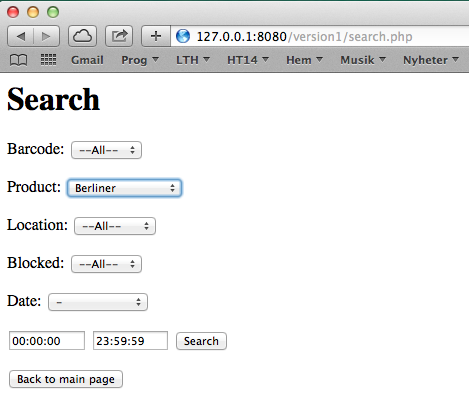
\includegraphics[width=\textwidth]{figures/view_search.png}
    	\label{figure:view_search}
    	\caption{View for searching}
 		\end{subfigure}	
 		\begin{subfigure}[b]{0.45\textwidth}
    	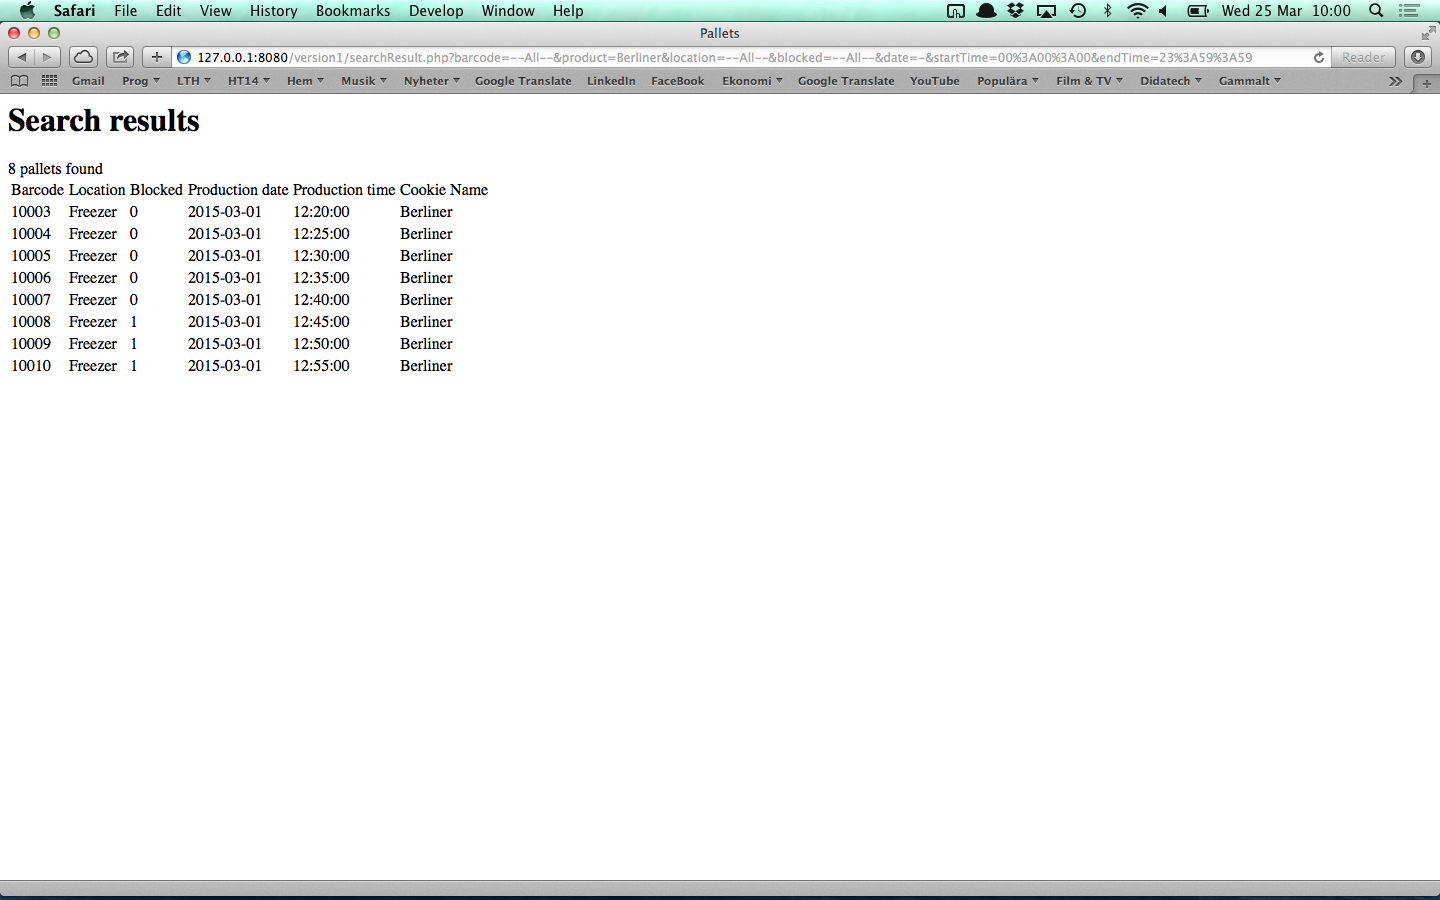
\includegraphics[width=\textwidth]{figures/view_searchResult.png}
    	\label{figure:view_searchResult}
    	\caption{Search results}
 		\end{subfigure} 
 		\caption{Views for searching}
\end{figure}


\subsection*{Blocking}

When the user wants to block pallets in a certain time intervall containing a certain product they can go to the block view. The user is the asked to choose which product they want to block and then a production date and time intervall to block all pallets with that product. The result of the request is the displayed in the next view. The user is provided with information on how many pallets that where blocked but also pallets in the intervall that are already blocked are displayed.

\begin{figure}[h]
  \centering
  	\begin{subfigure}[b]{0.45\textwidth}
    	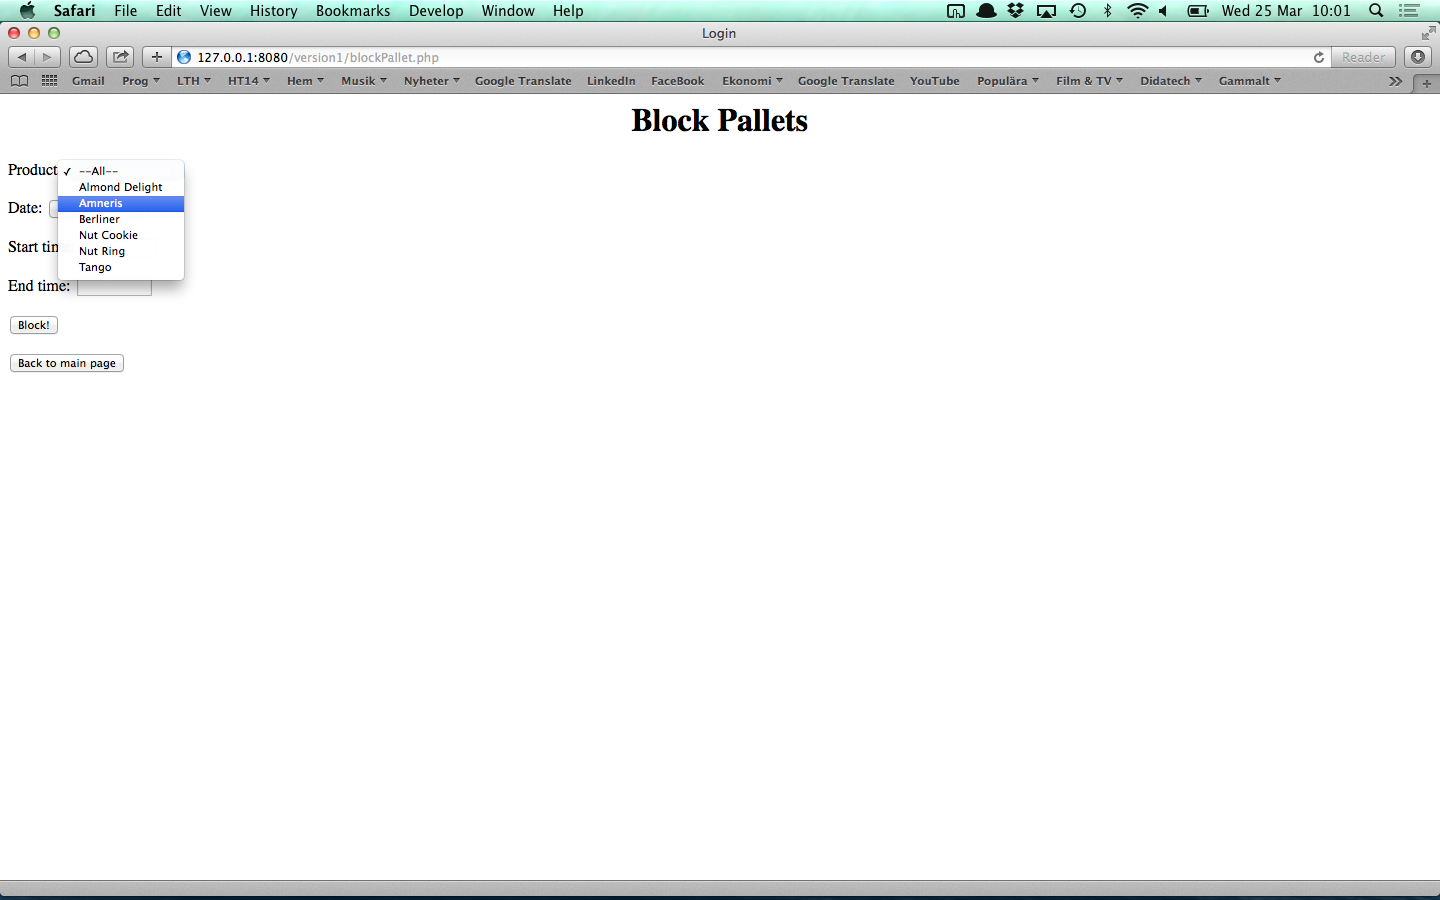
\includegraphics[width=\textwidth]{figures/view_block.png}
    	\label{figure:view_block}
    	\caption{View for choosing blocking conditions}
 		\end{subfigure}	
 		\begin{subfigure}[b]{0.45\textwidth}
    	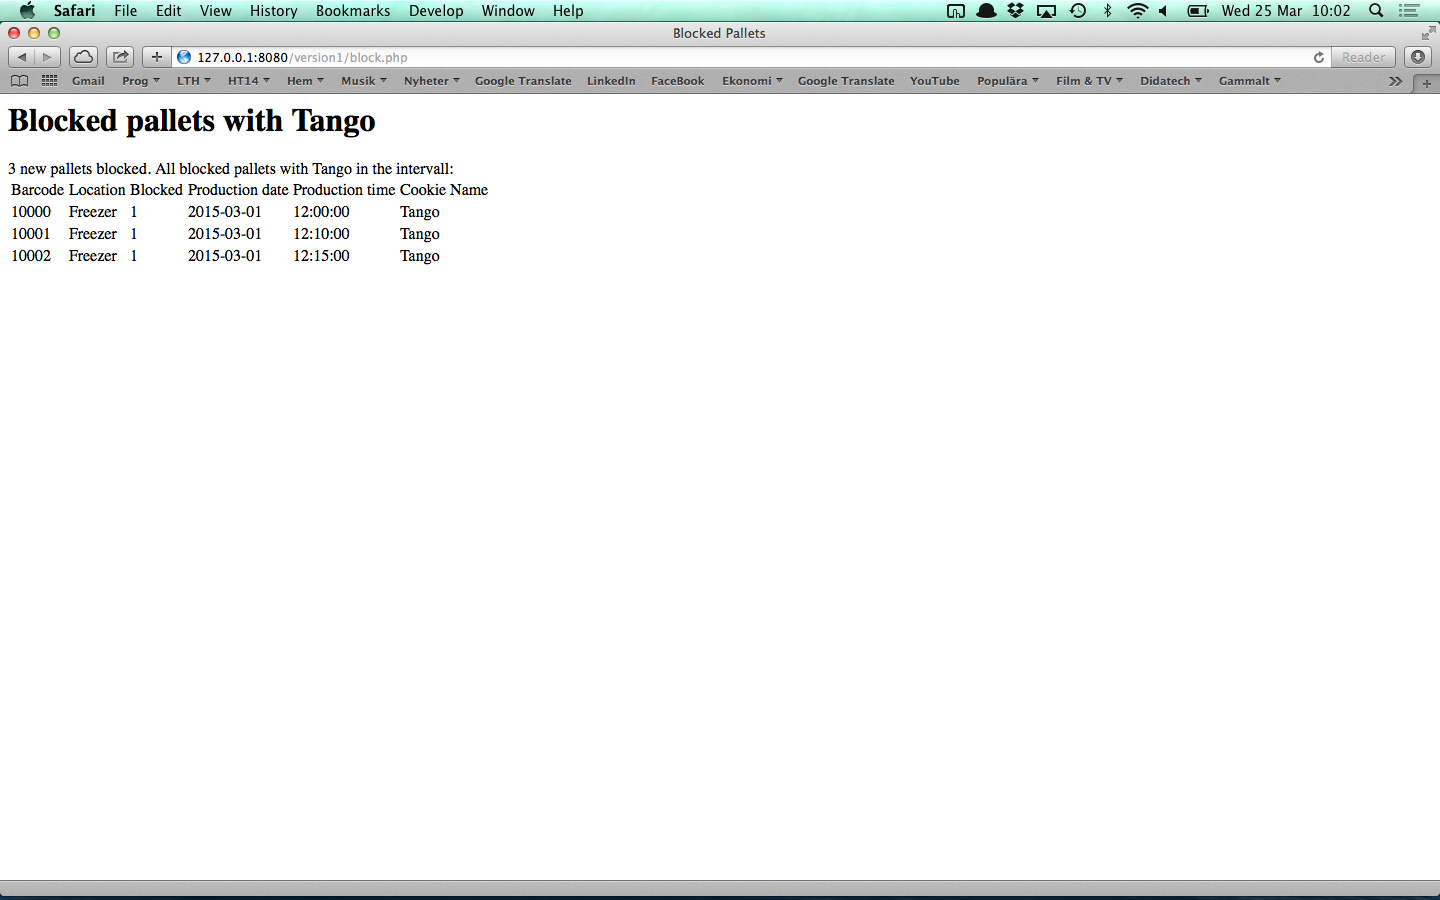
\includegraphics[width=\textwidth]{figures/view_blockResult.png}
    	\label{figure:view_blockResult}
    	\caption{Result view for blocking pallets}
 		\end{subfigure} 
 		\caption{Views for blocking pallets}
\end{figure}

\subsection*{Simulate production}

To simulate the production of a new pallet the user can enter a view where one can choose which product one wants to produce and then what date and time it should be done. The result can then be seen in the result if a pallet is produced is that the user get the barcode for the produced pallet back. The views can be seen below.

\begin{figure}[h]
  \centering
  	\begin{subfigure}[b]{0.45\textwidth}
    	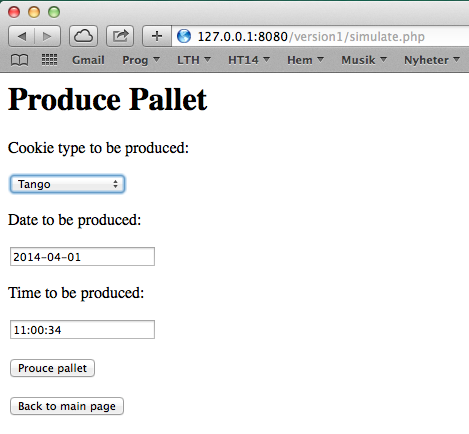
\includegraphics[width=\textwidth]{figures/view_produce.png}
    	\label{figure:view_produce}
    	\caption{Login view for the interface}
 		\end{subfigure}	
 		\begin{subfigure}[b]{0.45\textwidth}
    	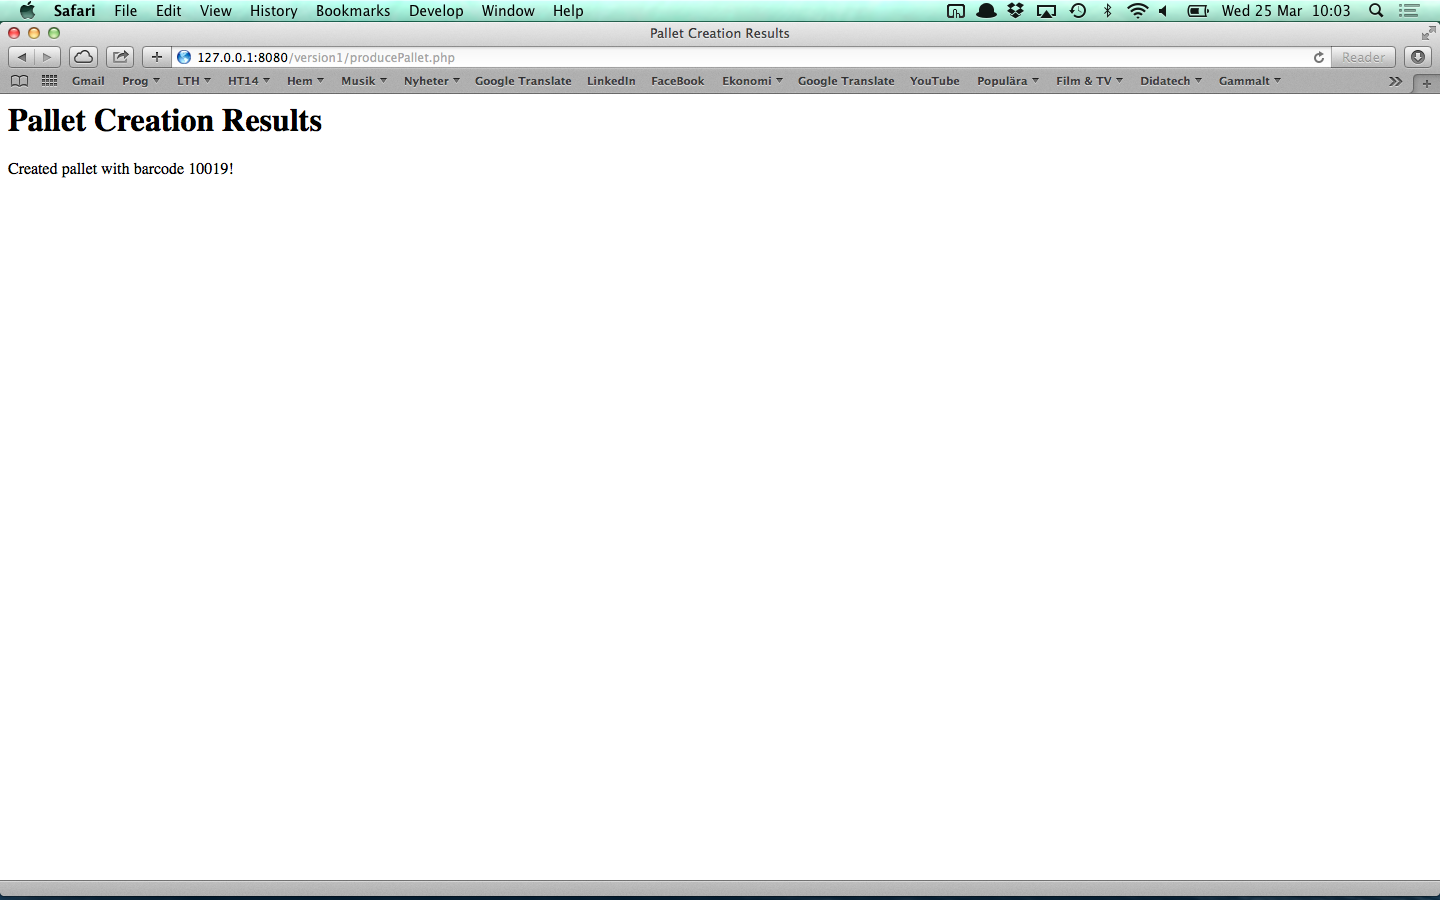
\includegraphics[width=\textwidth]{figures/view_produceResult.png}
    	\label{figure:view_produceResult}
    	\caption{View for the main page}
 		\end{subfigure} 
 		\caption{Views for simulated production}
\end{figure}

\section*{E/R Diagram}

\begin{figure}[h!]
  \begin{centering}
    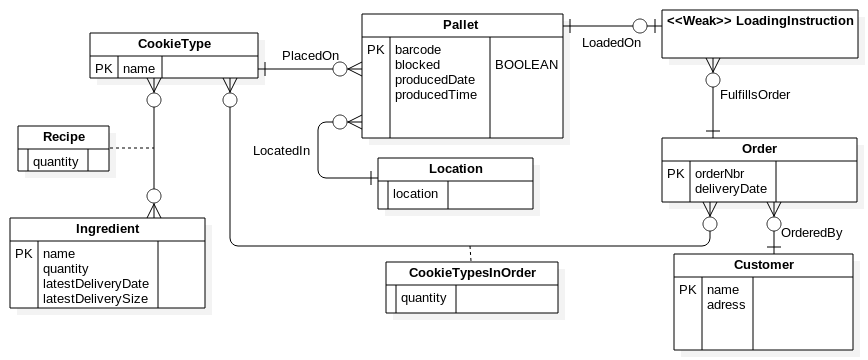
\includegraphics[width=\textwidth]{../ER.png}
    \label{er-diagram}
    \caption{E/R--diagram for the system}
  \end{centering}
\end{figure}

\section*{Relations}
The following relations were the basis for creating the database:

\lstinputlisting[label={Relations.txt},caption={Relations.txt},firstline=21]{../Relations.txt}
\section*{SQL Statements}
The following SQL statements were used to create the database:

\lstinputlisting[label={tables.sql},caption={tables.sql},lastline=83]{../tables.sql}
\section*{User's manual}
We consider the system self--explanatory enough not to require an user manual. 
The system has, in fact, been tested on a med--student with great success.
The only things worth pointing out are that:

\begin{enumerate}
  \item This thing
  \item This thing
  \item And this thing
\end{enumerate}

% \setcounter{section}{1}
% \section*{Task 1}
% \input{../task1/task1.tex}






% \begin{thebibliography}{9}
    
%   \bibitem{cb}
%     B. Kolman, R. E. Beck, \emph{Elementary Linear Programming with Applications}.
%     2nd edition. Academic Press, San Diego, 1995,

% \end{thebibliography}

\end{document}
